%!TEX root = ../mieic.tex


\chapter{Methodologies}
\label{chap:chap4}

\section*{}

In this chapter, further details about the methodologies used in the developed prototype, as well as in the the validation process, will be explored.

The development process will be compared to the previous expectations of the outcome of the planned prototype.

By this point, the validation of the prototype will be analysed, by explaining the performed user tests, as well the analysis of the results.


\section{Prototype} % (fold)
\label{sec:prototype}

  \subsection{Main Features} % (fold)
    \label{sub:main_features}
    
    The main features of RAMA's Spotify Application are: visualization of a map of a network of connected artists; edit the graph (expand and new map functions, as well as depth and branching parameters); Tags overlay and music artist info.

    \subsubsection{Visulization of the Artist Map} % (fold)
      \label{ssub:visualization}
    
      The application automatically draws the map with the current playing artist as the main node, as seen in Figure~\ref{fig:graph_rootnode}.

      \begin{figure}[tb]
        \begin{center}
          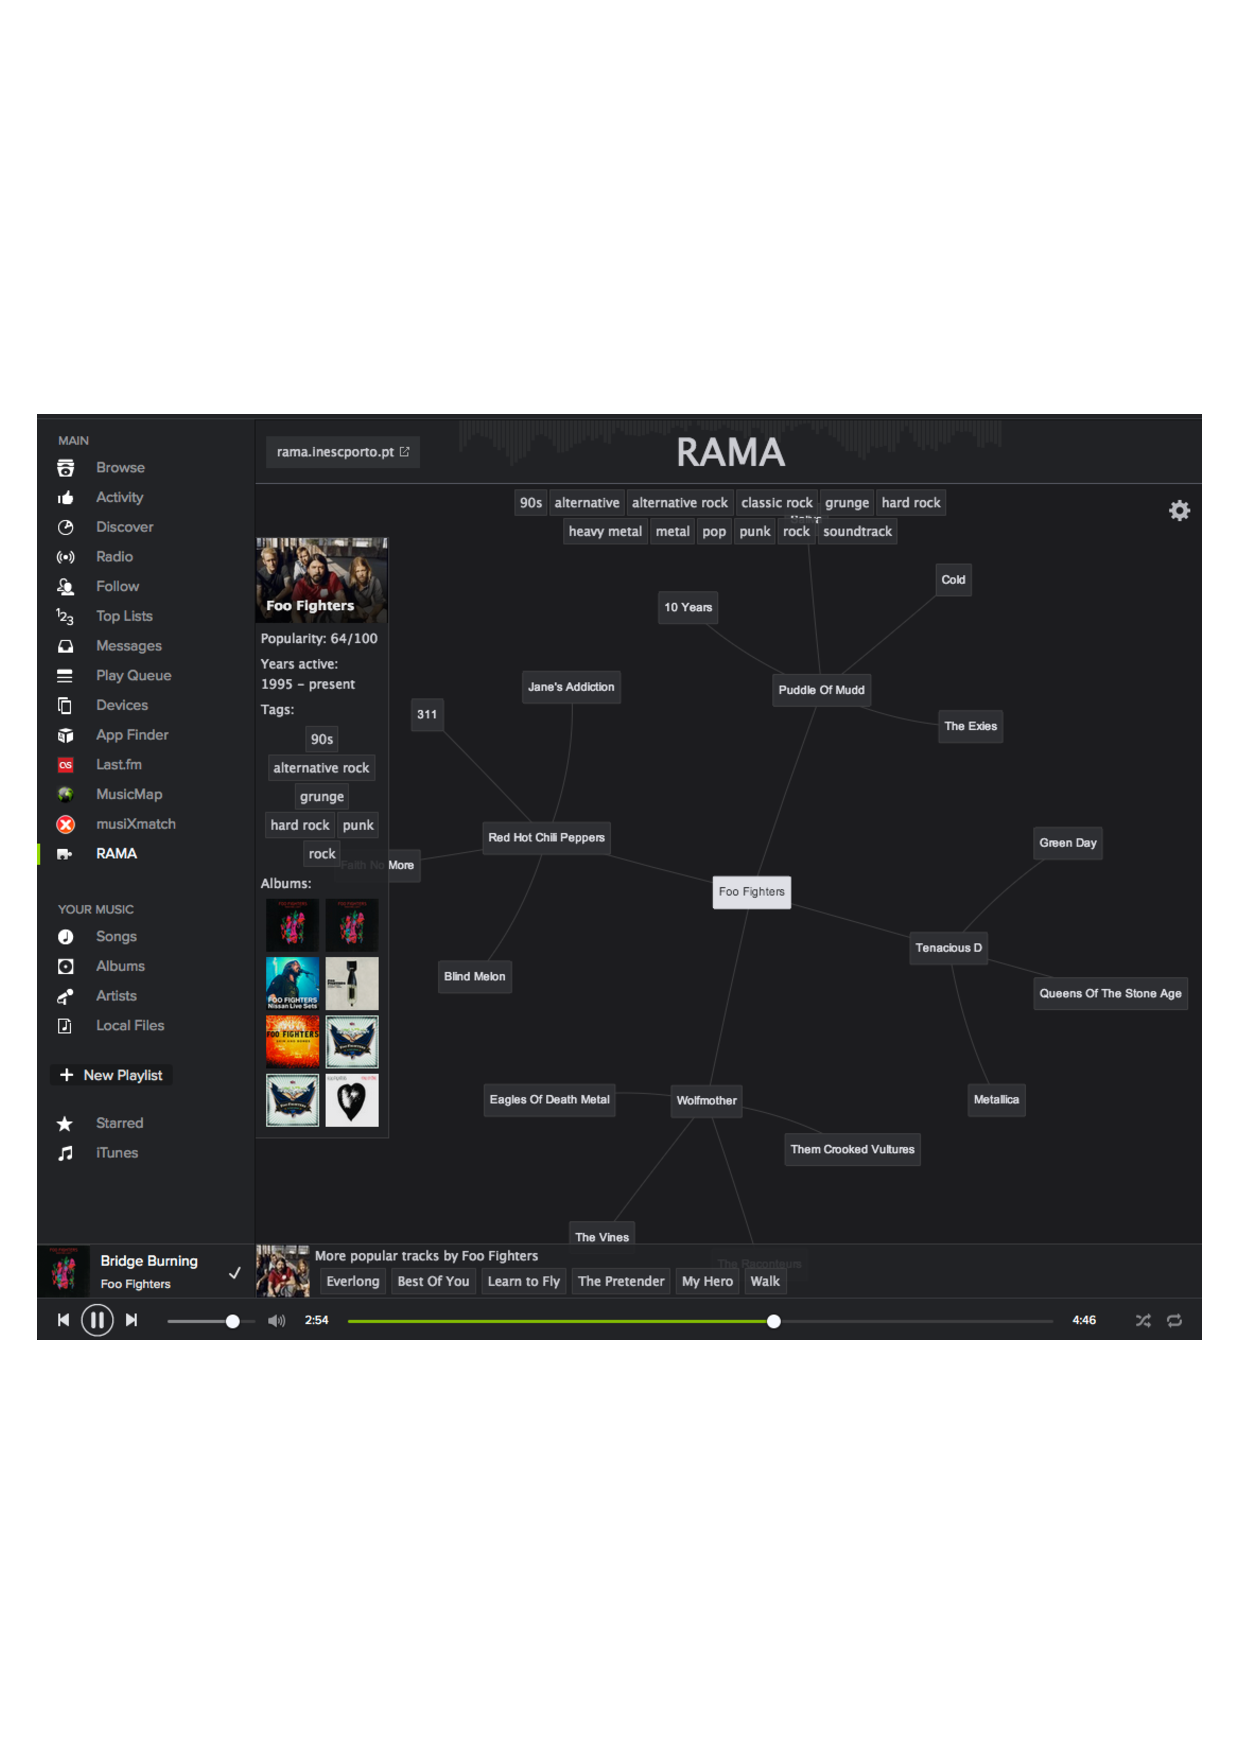
\includegraphics[width=\textwidth]{graph_rootnode.pdf}
        \end{center}
        \caption{The first drawn graph uses the current playing artist (lower left corner) as the root node.}
        \label{fig:graph_rootnode}
      \end{figure}

      The graph-like structure of the map, is created by recursively fetching a list of related artists from each artist. Once a certain pre-established limit of recursive levels is reached\footnote{depth value of a graph}, the algorithm stops.

      The graph creation algorithm is as follows:

      \lstinputlisting[
        caption={Simplified graph creation algorithm in Javascript (duplicate nodes checking is encapsulated in the insertNode function, as well as duplicate edges in the insertEdge function)}, style=htmlcssjs
      ]
      {snippets/map_creation_alg.js}

      This algorithm, albeit simplified, represents the basic flow when constructing a graph, or more specifically, a tree.
      Since that, in this case of study, the direction of the edges of the graph is not relevant in any way to the artists' map, all of the edges are considered to be undirected.

      Assuming that the insertNode() function only checks for duplicate nodes, i.e., it only inserts unique nodes into the graph, then the resulting graph is one of a tree, since there are no simple cycles in the graph.
      An example of this behaviour can be seen in Figure~\ref{fig:graph_treemode}.

      \begin{figure}[tb]
        \begin{center}
          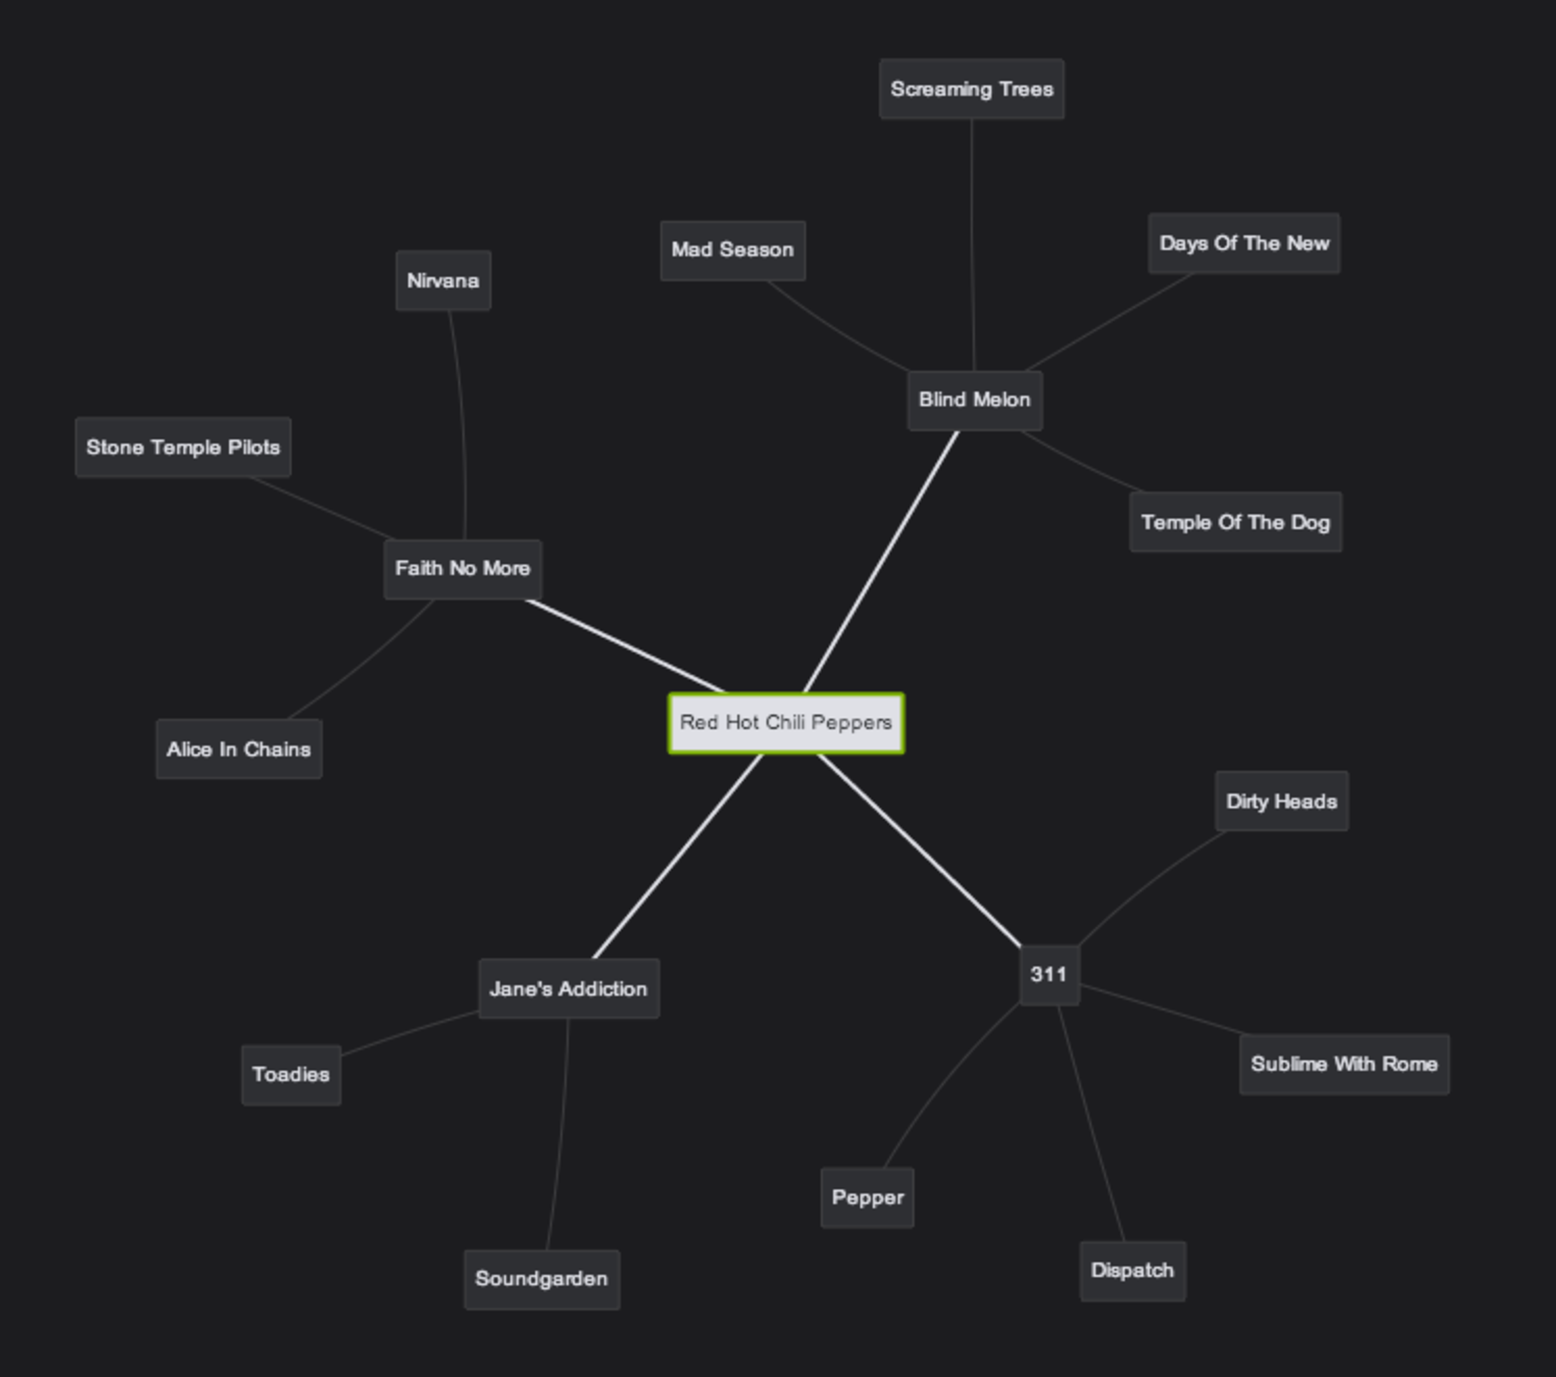
\includegraphics[width=\textwidth]{map_creation_treemode.pdf}
        \end{center}
        \caption{Graph created like a tree with "Red Hot Chilli Peppers" as the root node.}
        \label{fig:graph_treemode}
      \end{figure}

      This approach, however, is not showing all of the available information.
      Given this same example (Figure~\ref{fig:graph_treemode}), the artist node "Stone Temple Pilots" is a child of the node artist "Faith No More".
      The algorithm inserted the latter first into the graph.
      After that, when retrieving the childs of "Jane's Addiction", "Stone Templo Pilots" is contained in that list, and so the insertNode() function discards the node since it is a duplicate.
      But that means that there is a connection between the both of them that is being discarded.

      \hfill \\ 
      \noindent
      \textbf{Graph's Tree Mode}

      To build a graph with all the connections that exist between all of the artists in the graph, the insertNode() function would need to insert the missing edge into the graph by analysing the current graph state.
      This method creates a graph by definition, while the previous one created a tree graph.
      An example of this behaviour can be seen in Figure~\ref{fig:graph_notreemode}.
      \hfill \\
      \begin{figure}[tb]
        \begin{center}
          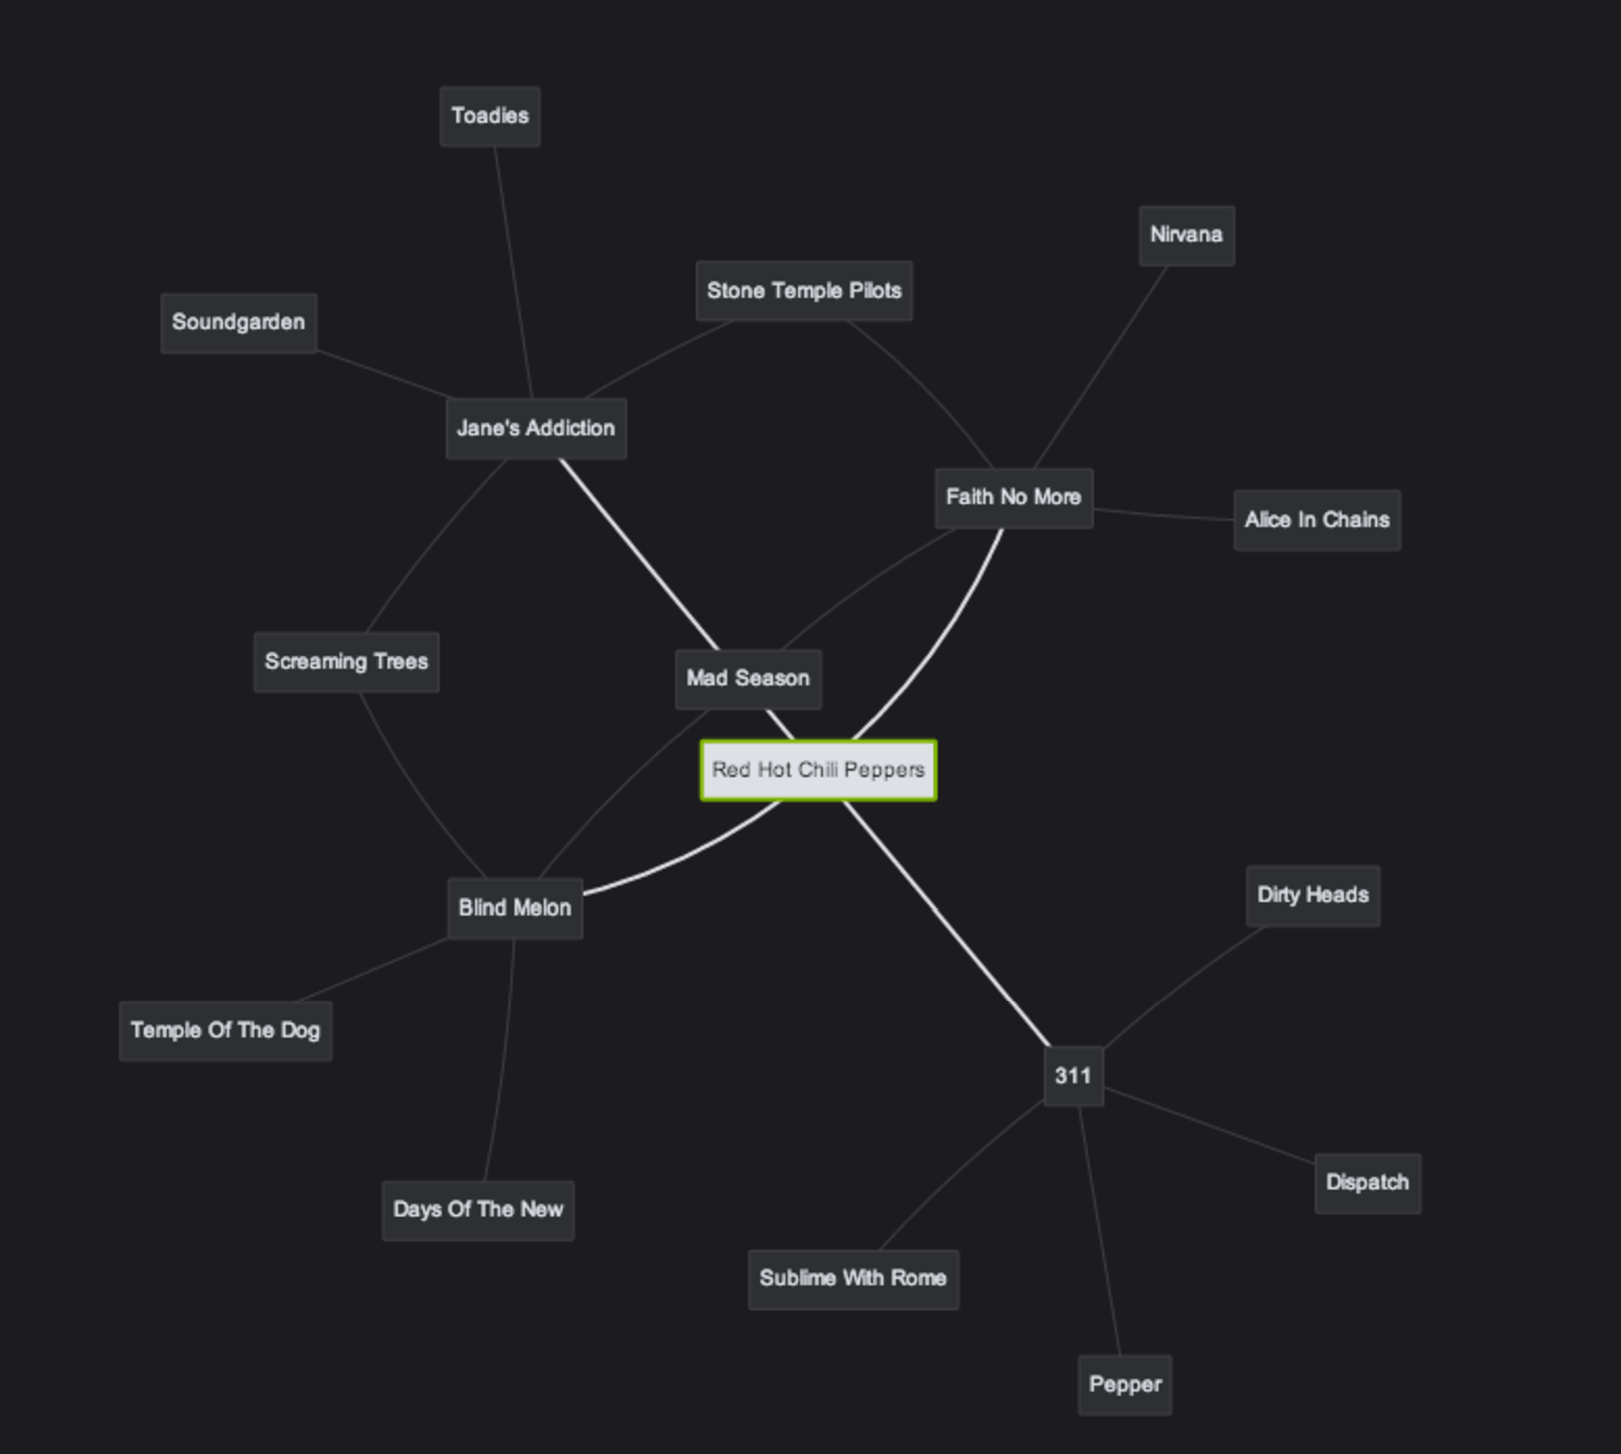
\includegraphics[width=\textwidth]{map_creation_notreemode.pdf}
        \end{center}
        \caption{Graph created with all the connections with "Red Hot Chilli Peppers" as the root node.}
        \label{fig:graph_notreemode}
      \end{figure}

      \emph{From now on, if the graph is a tree, it will be said that the algorithm is using the \emph{Tree Mode}.
            So the example \ref{fig:graph_treemode} is a \emph{Tree Mode} example, and the examples \ref{fig:graph_notreemode} and \ref{fig:graph_notreemode2} are not \emph{Tree Mode} examples\footnote{
              Note that, sometimes, even if the algorithm is not on tree mode, it might generate a tree, simply because there were no missing edges between the nodes to be added to the graph.
            }.}.
      \hfill \\

      Note (\ref{fig:graph_notreemode}) how "Stone Temple Pilots" is now child of both "Faith No More" and "Jane's Addiction".
      Also note that the same behaviour is visible with the nodes "Mad Season" and "Screaming Trees".

      In this case, the user's perception on the artist "Stone Temple Pilots" is now different from the previous example (Figure~\ref{fig:graph_treemode}).
      These added connections are, in a way, clustering together the most connected nodes.
      In this particular example, one could see an improvement with this approach: it contributes to the user's perception of the artist's network by making sure the user knows that those specific artists are more connected between them, than any others.

      \hfill \\
      \indent However, that is not always the case.

      The fact is, that in this example, only three extra edges where added, meaning there is not much visual clutter in the visualization.
      Although one could argue that the "Mad Season" artist node is already disturbing the visual representation by being drawn over an edge.

      With the exact same values of branching, depth and tree mode off, when creating a graph for the artist "Mariza", the visual clutter is so strong that the graph becomes confusing and not very helpful: Figure~\ref{fig:graph_notreemode2}.

      \begin{figure}[tb]
        \begin{center}
          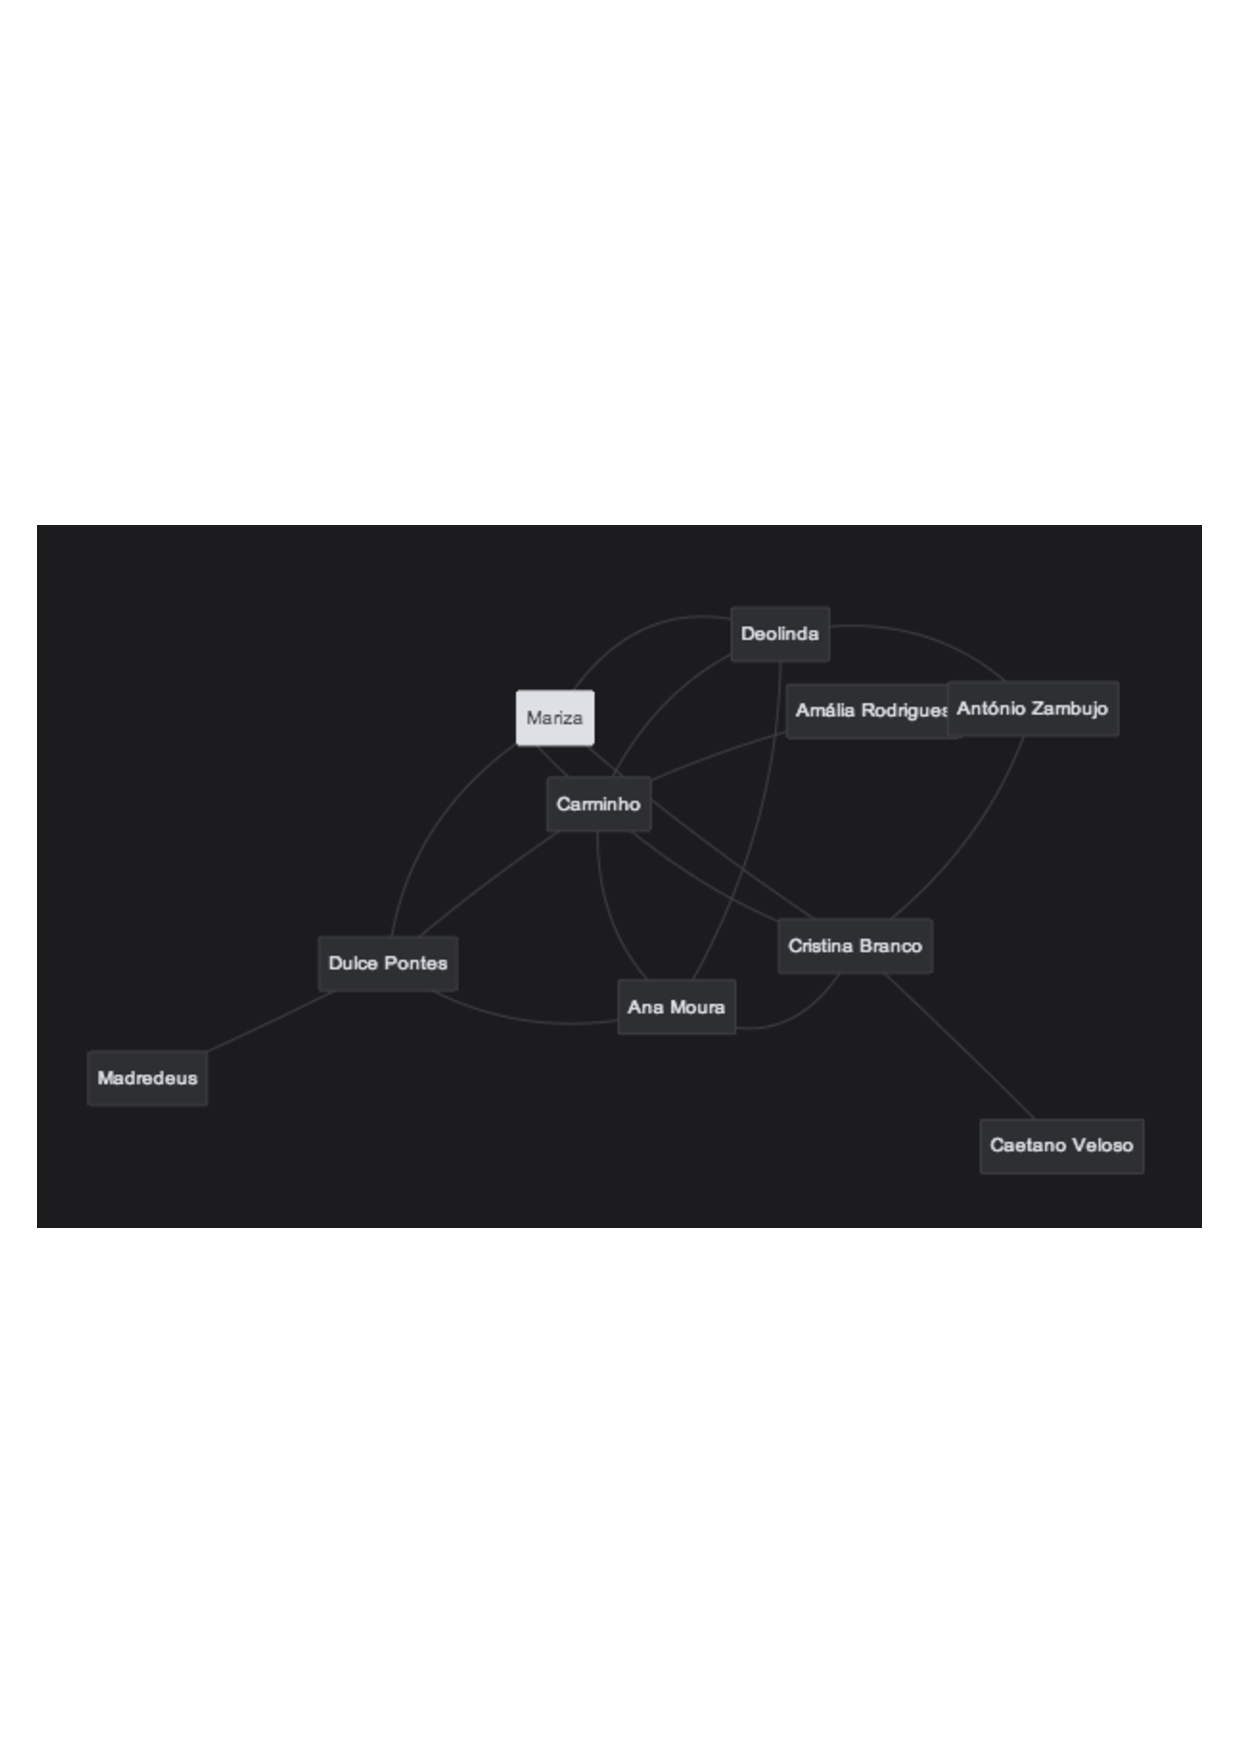
\includegraphics[width=\textwidth]{graph_notreemode2.pdf}
        \end{center}
        \caption{Graph created with all the connections with "Mariza" as the root node.}
        \label{fig:graph_notreemode2}
      \end{figure}

      The cluster of nodes in the center makes it clear that those specific nodes are really connected between them. 
      But then, the edges, that are forcing those nodes together, are creating a visual clutter that might not be so desirable.
      Instead of creating a visual map of the artists' network for the user to perceive, explore and change in its own way, the representation is more contained, static and not so visually appealing.
      \hfill \\

      So on one hand, the \emph{clustering} of the nodes seems like an interesting feature.
      It allows for a much more in-depth user access to the underlining information of the related artists.
      But on the other hand, the focus of the visualization (to show a map of the artists' network) was shifting to this cluster-like representation.

      Both perspectives are advantageous depending on the data they are operating on (as seen in the previous examples).
      So instead of choosing only one method, both were chosen: by default, the graph creation algorithm is on tree mode, and the user can turn it off from a settings menu.
      This allows for the user to choose the visual representation method that suits its needs.

      \paragraph{Depth and Branching values} \hfill \\

      The depth and branching values have been mentioned before in this chapter, but not further explained.

      The \textbf{depth} value of a graph


    % subsubsection visualization (end)

    \subsubsection{Graph Edition} % (fold)
      \label{ssub:edition}
    
    graph edition stuff

    % subsubsection edition (end)

    \subsubsection{Tags Overlay} % (fold)
      \label{ssub:tags_overlay}
    


    % subsubsection tags_overlay (end)

    \subsubsection{Artist Info} % (fold)
      \label{ssub:artist_info}
    


    % subsubsection artist_info (end)

  % subsection main_features (end)  


  \subsection{Development Process} % (fold)
    \label{sub:development_process}
  % subsection development_process (end)

% section prototype (end)


\section{Validation} % (fold)
\label{sec:validation}


  \subsection{User Tests} % (fold)
  \label{sub:user_tests}
  
  % subsection user_tests (end)

  \subsection{Data Analysis} % (fold)
  \label{sub:data_analysis}
  
  % subsection data_analysis (end)
% section validation (end)


\section{Conclusions} % (fold)
  \label{sec:conclusions}



% section conclusions (end)